\documentclass[12pt]{article}
\usepackage{pgfplotstable}
\usepackage[a4paper,margin=1in,landscape]{geometry}

\title{\bfseries Cup cooling experiment with Arduino}
\date{}
\begin{document}
\maketitle
\thispagestyle{empty}

\noindent
\textbf{Equipment}: \texttt{The K-type thermocouple with digital amplifier on the MAX6675 chip.}

\begin{center}
%---------------------------------------------------------
\begin{minipage}[]{0.45\linewidth}\centering
    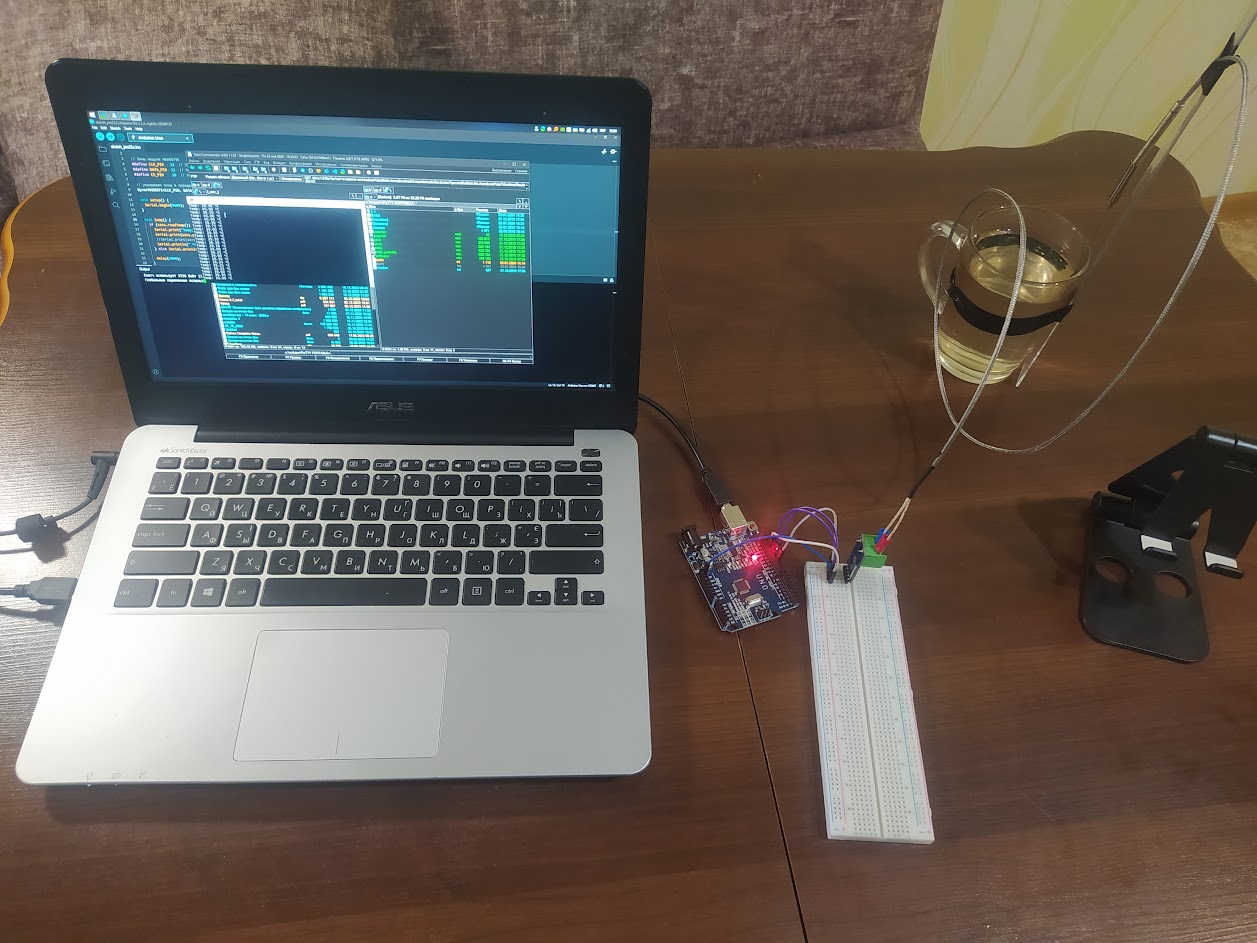
\includegraphics[width=\linewidth]{cooling.png}
\end{minipage}%
\quad
%---------------------------------------------------------
\begin{minipage}[]{0.45\linewidth}\centering
    \begin{tikzpicture}
    \begin{axis}[%
    title={Cooling a cup of tea},
    width=\linewidth,
    height=0.75\linewidth,
    			xlabel={$t$ / min},
    			ylabel={$T$ / ${^\circ}$C},
    scale only axis,
    enlargelimits=false,
    line join=round,
    % === Налаштування сітки ===
    grid = both,
    grid style={line width=.1pt, draw=gray!10},
    major grid style={line width=.2pt,draw=gray!50},
    minor tick num = 5,
    minor grid style = {line width=.1pt,draw=gray!10},
    ]
    \addplot [color=red, line width=1pt, mark=*, mark size=1pt] table [x expr=\coordindex * 5 / 60, y=y] {data.txt};



    \node[anchor=south east,
    		draw=none,
    		fill=white,
            font=\ttfamily\small,
    		align=left,
    		fill opacity=0.5,
    		text opacity=1,
    		] at ([shift ={(0cm,7cm)}]current axis.south east) {
    		Room temperature: $T_0 = 23^\circ$C\\
            Systematic absolute error of the sensor: $\pm 0.25^\circ$C
            };

    \end{axis}

    \end{tikzpicture}
\end{minipage}
%---------------------------------------------------------
\end{center}

%---------------------------------------------------------
\begin{figure}[h!]\centering
    \begin{tikzpicture}[%
    declare function={
    A = 24.530;
    B = 64.886;
    a = 0.09689;
    b = 0.00947;
    f(\x) = A * exp(-a*\x);
    g(\x) = B * exp(-b*\x);
    h(\x) = f(\x) + g(\x);
    },
    ]
    \begin{axis}[%
    title={Cooling a cup of tea},
    width=0.95\linewidth,
    height=0.5\linewidth,
    			xlabel={$t$ / min},
    			ylabel={$T$ / ${^\circ}$C},
    scale only axis,
    enlargelimits=false,
    line join=round,
    % === Налаштування сітки ===
    grid = both,
    grid style={line width=.1pt, draw=gray!10},
    major grid style={line width=.2pt,draw=gray!50},
    minor tick num = 5,
    minor grid style = {line width=.1pt,draw=gray!10},
    ]



    \addplot [only marks, color=red!50, mark=o, mark size=1pt] table [x expr=\coordindex * 5 / 60, y=y] {data.txt};

    \addplot [no markers, blue, ultra thick] gnuplot [raw gnuplot] {
                A = 90;
                C = 23;
                B = 0.1;
                a = 0.045;
                alpha = 1;
                f(x) = (A - C) * exp(-a * x ** alpha) + C;
%                g(x) = B * exp(-b * x);
%                h(x) = f(x) + g(x);
%                fit h(x) 'data.txt' u ($0 * 5 / 60):1 via A,C,B,a,b;
                fit f(x) 'data.txt' u ($0 * 5 / 60):1 via A,C,a,alpha;
%                plot [x=0:45] g(x);
                plot [x=0:45] f(x);
%                plot [x=0:45] h(x);
        };

%    \pgfmathsetmacro\A{A}
%    \pgfmathsetmacro\a{a}
%    \pgfmathsetmacro\B{B}
%    \pgfmathsetmacro\b{b}
%
%    \addlegendentry{Experiment}
%    \addplot [no markers, ultra thick, red, domain=0:45] {h(x)};
%    \addlegendentry{fit function $h(t) = f(t) + g(t)$}
%    \addplot [no markers, ultra thick, blue, dashed, domain=0:45] {f(x)};
%    \addlegendentry{$f(t) = \A\cdot e^{-\a\cdot t}$}
%    \addplot [no markers, ultra thick, brown, dashed, domain=0:45] {g(x)};
%    \addlegendentry{$g(t) = \B\cdot e^{-\b\cdot t}$}




    \end{axis}

    \end{tikzpicture}
%\caption{}
%\label{}
\end{figure}
%---------------------------------------------------------


\end{document}
